
\documentclass[pi.tex]{subfile}


\begin{document}
\chapter{TINJAUAN PUSTAKA}

Pada bab sebelumnya telah dijelaskan mengenai latar belakang dan tujuan dari penelitian yang akan dituliskan dalam penulisan ilmiah ini. Dengan mengacu pada bab sebelumnya, maka salah satu metode penelitian adalah dengan menggunakan tinjauan pustaka yang akan dijelaskan lebih lanjut pada bab ini.

\section{Komputasi Awan dan Amazon Web Service}
Seperti yang telah dijelaskan pada bab terdahulu, komputasi awan (\emph{cloud computing} atau biasa kita sebut \emph{cloud}  merupakan sebuah teknologi baru dalam dunia komputer khususnya dalam bidang sumber daya IT yaitu server. Hampir seluruh server yang digunakan oleh penyedia layanan teknologi informasi mulai memanfaatkan teknologi awan ini untuk mereduksi besaran biaya yang umumnya dikeluarkan apabila menggunakan arsitektur komputer tanpa awan. Di Indonesia, beberapa penyedia layanan IT baik berupa layanan ke konsumen maupun sesama penyedia jasa IT juga mulai melirik menggunakan teknologi awan ini. Sebagai contoh antara lain tokopedia.com, Go-Jek, bukalapak.com dan penyedia jasa IT lainnya berlomba-lomba untuk melakukan reduksi biaya yang timbul agar mendapat keuntungan maksimal dengan memindahkan sebagian infrastruktur IT nya ke layanan awan.

Selain dari sisi pengguna layanan komputasi awan, penyedia jasa komputasi awan publik sampai saat ini mulai tumbuh dan bersaing satu dengan lainnya untuk menarik perhatian konsumennya. Penyedia jasa komputasi awan publik antara lain, Amazon AWS, Google Cloud, Alibaba Cloud, yang berbasis penggunaan perjam, maupun DigitalOcean, Vultr, CloudKilat, yang berbasis penggunaan perbulan. Dalam penulisan kali ini yang jadi pembahasan adalah mengenai Amazon AWS atau dapat dikenal juga dengan nama \emph{Amazon Web Service}.

\subsection{Pengertian komputasi awan}
Komputasi awan adalah sebuah cara penyediaan dan penyaluran sumber daya komputer sesuai dengan yang diinginkan oleh pengguna dimana komputer-komputer yang digunakan tersebut berada pada media internet yang disediakan oleh penyedia jasa komputasi awan atau divisi internal IT sebuah perusahaan. Dalam dunia IT, komputasi awan kedalam tiga jenis cara pemasangan (\emph{type of deployments}), yaitu komputasi awan publik (\emph{public cloud}), komputasi awan privat (\emph{private cloud}), serta berdasarkan tipe layanan awannya terbagi kedalam tiga jenis yaitu IaaS (\emph{Infrastructure as a Service}), PaaS (\emph{Platform as a Service}), dan SaaS (\emph{Software as a Service}).

\subsubsection{Cara pemasangan \emph{cloud}}
Pemasangan infrastruktur IT khususnya komputasi awan terbagi kedalam dua jenis yaitu:

\begin{enumerate}
\item Komputasi Awan Publik
  Komputas awan publik merupakan jenis pemasangan \emph{cloud} yang disediakan oleh sebuah institusi penyedia layanan komputasi awan (\emph{Cloud Providers}) dimana dalam penyediaan sumber daya maupun cara pengaksesan sumber daya dapat dilakukan oleh seluruh pengguna secara luas. Yang dimaksud dengan pengguna secara luas adalah setiap pengguna baik dari individu maupun badan hukum secara bersama-sama menggunakan satu layanan komputasi awan yang disediakan oleh penyedia jasa tersebut.

  Dalam komputasi awan publik, pengguna menggunakan sumberdaya yang sama yang dimiliki oleh penyedia jasa. Pengguna yang dimaksud dapat berupa pengembang maupun pengusaha sebuah layanan aplikasi berbasis internet. Dengan penggunaan sumberdaya yang dilakukan secara bersama-sama, pengguna tidak perlu memikirkan untuk mempersiapkan perangkat keras yang dibutuhkan untuk menjalankan komputasi awan tersebut.
  
\item Komputasi Awan Privat
  Komputasi awan publik merupakan jenis pemasangan \emph{cloud} dimana pengguna dapat sekaligus merupakan penyedia jasa \emph{cloud} namun penyedia dalam lingkup internal. Komputasi awan privat diperlukan apabila pengguna ingin menggunakannya komputasi awan untuk kepentingan internal. Dengan menggunakan komputasi awan privat, pengguna harus menyediakan infrastruktur komputernya secara mandiri.
  Komputasi awan privat banyak digunakan oleh perusahaan-perusahaan berskala besar yang sudah memiliki pusat data tersendiri. Komputasi ini sangat menguntungkan karena biaya yang dikeluarkan menjadi lebih murah dibandingkan layanan komputasi awan publik.
\end{enumerate}
  

\subsection{Layanan \emph{Amazon Web Service} sebagai komputasi awan publik }

\emph{Amazon Web Service} atau biasa disingkat AWS, merupakan layanan penyedia jasa komputasi awan publik yang dibuat dan dikembangkan oleh perusahaan bernama Amazon, dimana perusahaan ini merupakan perusahaan \emph{E-Commerce} yang sangat terkenal di dunia. AWS dikembangkan Amazon pertama kali dikarenakan pada saat itu, Amazon melihat adanya peluang pengembangan suatu infrastruktur IT berbasis komputasi awan.

AWS yang pertama kali dikembangkan merupakan rangkaian uji coba Amazon untuk menguji coba performa komputasi awan. Di tahun 2006, Amazon mengubah seluruh infrastruktur IT nya yang semula masih berada di pusat datanya, kemudian dialihkan semuanya ke layanan AWS tersebut. Layanan AWS kemudian dipublikasikan kepada publik dan Amazon mulai memperdagangkan layanan AWS tersebut secara umum.

Pada saat ini, AWS memiliki lebih dari 20 layanan yang ditawarkan kepada konsumen untuk mereduksi biaya-biaya yang timbul apabila pengguna masih menggunakan infrastruktur dengan cara konvensional. Layanan AWS yang paling terkenal adalah EC2 (\emph{Elastic Cloud Computing}), ELB (\emph{Elastic Load Balancer}), dan AWS Lambda. Layanan AWS seluruhnya diberikan dengan skema pembayaran penggunaan per jam ataupun hitungan arus jaringan yang diterima oleh layanan AWS tersebut.

Dari seluruh penyedia jasa layanan komputasi awan publik, AWS menduduki peringkat yang paling tinggi dari kategori pendapatan dan performa. Layanan AWS sampai saat ini belum bisa disaingi oleh layanan komputasi awan publik lainnya.

\section{Bahasa Pemrograman Fungsional dan Metode Pemrograman Fungsional Reaktif}
Dalam pembuatan sebuah software, pemilihan bahasa pemrograman merupakan salah satu hal yang mempengaruhi program yang akan dikembangkan. Bahasa pemrograman menjadi kunci dari sebuah program dikarenakan dengan bahasa pemrograman itulah, manusia dapat berinteraksi dengan komputer. Hal ini dikarenakan bahasa pemrograman menjadi alat translasi dari bahasa manusia ke mesin. Dalam perkembangannya, lingkup bahasa pemrograman dibagi menjadi 3 (tiga) yaitu bahasa pemrograman terstuktur (\emph{imperative programming}), bahasa pemrograman berorientasi objek (\emph{object oriented programming}), dan bahasa pemrograman fungsional (\emph{functional programming} atau biasa disebut juga sebagai \emph{declarative programming}).

Selain lingkupnya, setiap bahasa pemrograman memiliki metode dalam setiap penulisannya. Metode ini diperlukan sebagai acuan bagi pemrogram untuk membuat sebuah software yang memiliki kemampuan dan performa yang baik. Metode dari bahasa pemrograman tersebut juga digunakan untuk memastikan tidak adanya kegagalan sistem maupun error yang terbentuk dari program yang dijalankan. Dalam sub bab ini akan dijelaskan lebih lanjut mengenai teori-teori pendukung yang digunakan dalam penulisan ilmiah diantaranya teori pemrograman fungsional, Haskell, \emph{Glasgow Haskell Compiler} atau GHC, FRP, Reflex dan Reflex-dom.

\subsection{Pemrograman Fungsional}
Pemrograman fungsional adalah merupakan salah satu dari paradigma dalam pemrograman. Paradigma pemrograman adalah kumpulan dari konsep yang digunakan oleh suatu bahasa pemrograman (Serrano Mena, hlm. 4). Paradigma yang digunakan oleh pemrograman fungsional adalah paradigma yang bergantung pada pemodelan sebuah fungsi matematika. Sebagai contoh, fungsi sederhana dari matematika yang banyak diketahui adalah sebagai berikut:

\begin{equation}
  f(n) = n^3 + 4n^2 + 2
\end{equation}

Dalam hal ini pemrograman fungsional merupakan sebuah gabungan ekspresi dalam pemodelan matematika, dimana termasuk didalamnya adalah nilai konkrit, variabel, dan juga bisa dalam bentuk fungsi lainnya. Sedangkan fungsi seperti pada contoh diatas, adalah merupakan ekspresi yang dapat menerima sebuah argumen atau input, dan ketika menerima input tersebut, fungsi dapat terevaluasi atau tereduksi menjadi fungsi berikutnya.

Selain itu, pemrograman fungsional memperlakukan fungsi sebagai \emph{first-class} atau kelas utama dalam struktur pemrogramannya. Hal ini berarti, dalam pemrograman fungsional, sebuah fungsi dapat dimanipulasi layaknya tipe data lain dalam program. Fungsi dapat digunakan sebagai argumen atau input bagi fungsi lainnya, mengembalikan hasil dan atau disimpan kedalam sebuah variabel. Kemampuan untuk memperlakukan fungsi sebagai data memungkinkan adanya abstraksi tingkat tinggi sehingga memungkinkan untuk digunakan kembali.

Dengan demikian, secara umum dapat ditarik kesimpulan bahwa pemrograman fungsional dapat dilihat sebagai gaya pemrograman yang metode dasar komputasinya adalah pengaplikasian fungsi kedalam argumennya [5](Graham Hutton, hlm. 4). Contohnya, apabila ada fungsi $f(x) = 1 + x$ maka aplikasi fungsi terhadap nilai 1 adalah $f(1) = 1 + 1$ dan menghasilkan nilai keluaran 2. Hal yang menjadi inti dan paling krusial dari sebuah pemrograman fungsi adalah bahwa fungsi merupakan hubungan antara himpunan masukan dan keluaran [2](Chris Allen, hlm. 3), dimana setiap masukan maka akan menghasilkan keluaran yang selalu sama. Contohnya apabila $f(1) = A$, $f(2) = B$ maka apabila fungsi tersebut diaplikasikan dengan nilai yang sama (yaitu 1), hasil dari fungsi tersebut adalah tetap A. Sehingga, apabila ada fungsi $f(1) = A$ dan $f(2) = B$, maka dapat dikatakan notasi tersebut bukanlah sebuah fungsi.



\subsection{Sejarah Singkat Haskell}
Setelah dirilisnya bahasa dengan nama Miranda pada tahun 1985 oleh Research Software Ltd, ketertarikan pemrogram dengan bahasa pemrograman fungsional semakin meningkat. Pada tahun 1987, lebih dari 10 bahasa pemrograman fungsional ada. Berdasarkan konferensi \emph{Functional Programming Languages and Computer Architecture} di Portland, Oregon, sebuah meeting diadakan oleh sebuah komite untuk membentuk suatu bahasa pemrograman fungsional yang dapat digunakan oleh banyak pihak.

Bahasa pemrograman Haskell kemudian dikembangkan oleh Simon Peyton Jones dan beberapa rekannya yang tergabung dalam sebuah komite, ketika ia melakukan riset di sebuah institusi riset milik microsoft (\emph{Microsoft Research Institution}). Kemudian pada tahun 2003, komite Haskell berhasil merilis sebuah laporan (\emph{Haskell Report}) yang menjelaskan secara rinci mengenai versi stabil dari Haskell sehingga layak untuk digunakan.

Pada tahun 2010, komite Haskell mengeluarkan laporan kembali yang berisikan berbagai standarisasi dan perkembangan dari pengembangan bahasa Haskell. Hingga sekarang, standarisasi tersebut menjadi acuan bagi kompiler dan pengembang dalam mengembangkan aplikasi menggunakan bahasa Haskell (standarisasi tersebut dikenal dengan Haskell2010).

Hingga tahun 2017, banyak industri-industri bisnis di dunia yang menggunakan Haskell sebagai bahasa pendukung usahanya seperti Bank ABN Amro, Barclays Capital Quantitative Analytics Group, Facebook, Google, Intel, Microsoft, DATA61, NVIDIA, Bank Standard Chartered, dan masih banyak lainnya. Hal ini membuktikan bahwa penggunaan bahasa pemrograman fungsional untuk pengembangan aplikasi program pada skala industri sangat dimungkinkan.


\subsection{Fitur Haskell dan Pembuatan Program dengan Bahasa Haskell}

Sebagaimana dijelaskan sebelumnya, Haskell merupakan bahasa pemrograman yang sangat bergantung pada fungsi seperti fungsi pada matematika. Oleh karena itu, bahasa haskell cocok untuk digunakan dalam mengembangkan sebuah aplikasi karena sangat jarang menimbulkan masalah dikemudian hari. Haskell juga disebut sebaga bahasa pemrograman fungsional yang murni, dimana dalam penulisannya untuk membuat program, tidak ada konsep OOP sama sekali, dan seluruh tipe datanya merupakan sebuah fungsi. Bahasa pemrograman yang tidak murni fungsional antara lain, Kotlin, Scala, Ocaml, dan lain-lain.

Pengembangan aplikasi dengan menggunakan bahasa pemrograman fungsional yang murni seperti Haskell dapat membantu tingkat pemeliharaan aplikasi tersebut. Hal ini dikarenakan Haskell sebagai bahasa pemrograman fungsional yang murni memiliki beberapa fitur yang akan dijelaskan sebagai berikut.

 \subsubsection{\emph{Type System} yang kuat}
  
  Pendefinisian dari \emph{type system} sangatlah sulit dilakukan, dikarenakan banya para ahli yang memiliki pandangan berbeda satu sama lain. Menurut Benjamin C. Pierce dalam bukunya \emph{Types and Programming Language}, \emph{type system} adalah metode sintaksis yang mudah digunakan untuk membuktikan ketiadaan perilaku sebuah program dengan menggolongkan frase berdasarkan jenis dari nilai yang dikomputasi oleh prgram tersebut [2](Benjamin C. Pierce, hlm. 1). Haskell memiliki \emph{type system} yang sangat kuat sehingga deteksi galat pada program dapat diketahui pada saat program dikompilasi atau dapat dideteksi dini atas tipe data sebuah fungsi pada saat program sedang dikompilasi. Hal ini menjadikan galat program dapat sangat diminimalisasi untuk terjadi pada fase \emph{runtime} atau dikenal dengan \emph{runtime errors}.

  \emph{type system} pada haskell telah dikembangkan dalam waktu bertahun-tahun untuk memberikan fleksibilitas, pemeriksaan statis yang ekspresif dengan bantuan dari para peneliti untuk mengidentifikasi teknik-teknik \emph{type system} yang dapat menjadikan kelas-kelas baru terverifikasi dengan baik saat waku kompilasi (\emph{compiled time verification}). Untuk dapat lebih menjelaskan keunggulan dari \emph{type system} pada haskell, maka perlu diberkan contoh perbandingan antara Haskell dan C++.

  Pada Haskell, tipe data Maybe dideklarasikan sebagai berikut:\\
  \begin{lstlisting}[language=Haskell]
    data Maybe a = Nothing | Just a
  \end{lstlisting}
  dimana maksud dari tipe data tersebut adalah tipe data \fhaskell{Maybe} memiliki dua nilai kemungkinan yaitu Nothing atau \fhaskell{Just a}, dimana variabel \fhaskell{a} merupakan variabel abstrak yang biasa disebut \emph{polymorphic variable} yang dapat berupa tipe data lain. Selanjutnya untuk membuat tipe data yang sama pada C++, maka dapat dideklarasikan sebagai berikut:\\
  \begin{lstlisting}[language=C++]
    template <T>
    struct Maybe {
        bool isJust;
        T value;  // IMPORTANT: must ignore when !isJust
    };
  \end{lstlisting}

  Dari kedua deklarasi diatas, maka tipe data tersebut dapat digunakan untuk deklarasi fungsi sebagai berikut:

  Pada Haskell:\\
  \begin{lstlisting}[language=Haskell]
    sumJusts :: Num a => [Maybe a] -> a
  \end{lstlisting}

  Pada C++:\\
  \begin{lstlisting}[language=C++]
    template <T> T sumJusts(vector<maybe<T> >);
  \end{lstlisting}

  Dari kedua fungsi tersebut, dapat dibandingkan bahwa deklarasi fungsi pada C++ dimungkinkan terjadinya kesalahan karena tidak adanya \emph{type system} yang menyatakan bahwa fungsi tersebut membutuhkan \fhaskell{(+)} dan dijalankan dari angka 0. Sementara pada fungsi yang dideklarasikan dengan bahasa Haskell, maka kode \fhaskell{Num a =$>$} menjadi acuan bagi \emph{compiler} untuk memberitahukan bahwa tipe data masukan haruslah merupakan bagian dari tipe kelas \fhaskell{Num}. Hal ini akan menjadikan pesan galat yang muncul ketika melakukan kompilasi sangat ringkas dan jelas.

  Selain dari contoh yang telah disebutkan diatas, fitur pada \emph{type system} yaitu \emph{type inference} yaitu kemampuan bahasa Haskell untuk menentukan sendiri tipe fungsi (\emph{function signature}) yang ada pada sebuah fungsi apabila penulis kode program tidak memberikan tipe fungsi secara eksplisit. Hal ini sangat memudahkan pengembang untuk memeriksa tipe fungsi hanya dari deklarasi fungsinya tersebut.

 \subsubsection{Program yang \emph{Concise}}
  
  \emph{Concise} atau ringkas merupakan keunggulan Haskell. Hal ini disebabkan karena Haskell memiliki tingkat abstraksi tingkat tinggi dalam konsep pemrogramannya dimana jumlah sintak yang digunakan untuk menulis program dengan Haskell dibanding bahasa pemrograman lain lebih sedikit. Sebagai contohnya adalah penulisan fungsi pencarian fibbonaci dalam Haskell dan C++:\\

  Bahasa Haskell: 
  \begin{lstlisting}[language=Haskell]
    fib_rec 0 = 0
    fib_rec 1 = 1
    fib_rec n = fib_rec (n-1) + fib_rec (n-2)  
  \end{lstlisting}


  Bahasa C++:
  \begin{lstlisting}[language=C++]
    #include <iostream>  
  
    using namespace std;  
  
    int main() {  
       int number[30] = {1, 1, 0};  
       int total;  
       for (int i = 2; i < 30; i++) {  
         number[i] = number[i - 1] + number[i - 2];  
         cout << number[i] << endl;  
       }  
       return 0;  
     }  
  \end{lstlisting}

  Berdasarkan contoh diatas, Haskell memungkinkan pengembang untuk menuliskan jumlah kode yang lebih sedikit. Selain itu, alur logika yang dibentuk dari kode program tersebut sangat memudahkan pengembang untuk mengetahui bagaimana sebuah fungsi bekerja. Dari contoh tersebut dapat dengan mudah diketahui bahwa fungsi \fhaskell{fibbonnaci} diatas apabila diberikan input parameter 0 maka hasilnya 0, lalu apabila diberikan input dengan nilai 1 maka hasilnya 1, dan apabila diberikan input bernilai n, maka akan dilakukan fungsi rekursi yang mengeksekusi dirinya sendiri sampai nilai n tersebut bernilai 0 atau 1.

  Hal ini sangat membantu tidak hanya untuk kemudahan perawatan kode program melainkan apabila pengembangan aplikasi dilakukan secara berkelompok. Dengan penulisan struktur kode yang ringkas, pengembang lain sangat mudah untuk membaca kode dan menganalogikan alur pemikiran dari aplikasi yang dikembangkan oleh pengembang aslinya.

  Contoh lain yang menjadikan Haskell sebagai program yang ringkas dapat dilihat pada contoh potongan kode sebagai berikut:\\
  \begin{lstlisting}[language=Haskell]
    ganjil = [1,3..100]
    genap = [2,4..100]
    genap2 = [x | x <- [1..100], x `mod` 2 == 0]
  \end{lstlisting}
  kode diatas adalah untuk mendaklarasikan kumpulan angka genap dan ganjil dalam sebuah tipe data \fhaskell{List} (atau biasa direpresentasikan dengan notasi \fhaskell{[ ]}) atau Array pada bahasa pemrograman berorientasi objek pada umumnya. Pada Haskell dimungkinkan penggunaan \emph{List Comprehension} dimana kemampuan deteksi kompiler terhadap isi dari elemen pada \fhaskell{List} menggunakan notasi yang mendekati notasi deklarasi himpunan pada Matematika. Contoh deklarasi \emph{List Comprehension} adalah pada variabel \fhaskell{genap2} diatas. Dari notasi tersebut dapat dibahasakan bahwa variabel \fhaskell{genap2} adalah kumpulan elemen pada \fhaskell{List} dimana terdiri dari \fhaskell{x} yang terdiri dari bilangan 1 sampai 100, dan \fhaskell{x} tersebut apabila dioperasikan dengan modulo 2 harus sama dengan 0. Perlu diberi catatan bahwa \fhaskell{x} yang merupakan sebuah abstraksi tipe data yang menandakan elemen dari \fhaskell{List} tersebut memiliki tipe data yang sama, dimana syarat dari \fhaskell{List} pada Haskell adalah memiliki elemen dengan tipe data yang sama.

\subsubsection{Fungsi Rekursi}
  
Banyak konsep perulangan di dalam bahasa pemrograman pada umumnya. Konsep pengulangan yang dimiliki Haskell adalah dengan menggunakan fungsi rekursi dimana penulisan kode akan lebih singkat dan lebih cepat dibandingkan perulangan biasa dalam bahasa pemrograman fungsional. Contoh dari proses rekursi pada haskell telah dijelaskan sebelumnya yaitu pada potongan kode yang berisikan fungsi bilangan fibbonacci diatas. Perulangan secara rekursi pada Haskell sangat banyak digunakan pada fungsi-fungsi standar. Sebagai contoh untuk membalikkan sebuah kata "andika", maka dapat digunakan fungsi bawaan (\emph{in-built function}) \fhaskell{reverse} dimana deklarasi dari fungsi ini adalah sebagai berikut:\\

  \begin{lstlisting}[language=Haskell]
    reverse :: [a] -> [a]  
    reverse [] = []  
    reverse (x:xs) = reverse xs ++ [x] 
  \end{lstlisting}

  Dari fungsi diatas maka dapat dianalogikan bahwa kata "andika" memiliki tipe data \fhaskell{String}, yaitu kumpulan dari tipe data \fhaskell{Char} sehingga dapat ditulis juga menjadi tipe data \fhaskell{[Char]}. Hal ini sesuai dengan tipe fungsi dari reverse yaitu menerima parameter masukan berupa \fhaskell{[a]}, dan variabel \fhaskell{a} disini adalah tipe data polimorpisme dan \fhaskell{Char} adalah termasuk dari bagian tipe data yang dimaksud pada \fhaskell{a} tersebut. Kemudian, fungsi \fhaskell{reverse} akan dijalankan pada kata "andika" dengan cara berurut seperti pada kode berikut:\\

  \begin{lstlisting}[language=Haskell]
    reverse ['a','n','d','i','k','a']
    reverse ('a':['n','d','i','k','a']) = (reverse ['n','d','i','k','a']) ++ ['a']
    reverse ('n':['d','i','k','a']) = (reverse ['d','i','k','a']) ++  ['n'] ++  ['a']
    reverse ('d':['i','k','a']) = (reverse ['i','k','a']) ++  ['d'] ++  ['n'] ++  ['a']
    reverse ('i':['k','a']) = (reverse ['k','a']) ++  ['i'] ++  ['d'] ++  ['n'] ++  ['a']
    reverse ('k':['a']) = (reverse ['a']) ++ ['k'] ++ ['i'] ++  ['d'] ++  ['n'] ++ ['a']
    reverse ('a':[]) = (reverse []) ++ ['a'] ++  ['k'] ++  ['i'] ++  ['d'] ++  ['n'] ++  ['a']
    reverse [] = [] ++ ['a'] ++  ['k'] ++  ['i'] ++  ['d'] ++  ['n'] ++  ['a']
    reverse [] = ['a','k','i','d','n','a']
  \end{lstlisting}

  Dari ilustrasi tersebut, maka fungsi rekursi memudahkan untuk melakukan terhadap manipulasi berbagai tipe data untuk kepentingan pembuatan program.

  \subsubsection{\emph{High-order Functions}}
  
  Seperti dalam matematika, fungsi dalam Haskell dapat digunakan sebagai argumen atau inputan dalam fungsi lain dan fungsi dapat juga dikomposisikan dengan fungsi lainnya sebagaimana fungsi komposisi bekerja pada matematika.  \emph{High-order Functions} atah HOF ini yang menjadikan Haskell sangat \emph{powerfull} dibandingkan bahasa pemrograman pada umumnya. Hal ini dapat diilustrasikan dengan potongan kode program seperti dibawah ini:\\
  \begin{lstlisting}[language=Haskell]
    jadikanDuaKali :: (a -> a) -> a -> a  
    jadikanDuaKali f x = f (f x) 
  \end{lstlisting}

  Hal yang menandakan bahwa sebuah parameter adalah merupakan sebuah fungsi adalah penggunaan tanda kurung \fhaskell{()} pada deklarasi tipe fungsi. Dari fungsi diatas, maka fungsi \fhaskell{jadikanDuaKali} membutuhkan sebuah parameter dengan tipe \fhaskell{(a -> a)} yang merupakan sebuah fungsi. Penggunaan \emph{high order function} pada kode diatas dapat ditampilkan sebagai berikut:\\

  \begin{lstlisting}[language=Haskell]
    jadikanDuaKali (+3) 10 == 16
    jadikanDuaKali (++ " HOHO") "HI" == "HI HOHO HOHO"
  \end{lstlisting}

Dengan demikian, fitur ini sangat memungkinkan eksekusi terhadap suatu fungsi akan ditentukan dari hasil eksekusi fungsi lainnya sehingga menjadikan sebuah program akan lebih modular.

\subsubsection{\emph{Lazy Evaluation}}
  
\emph{Lazy evaluation} adalah sebuah konsep dimana tidak perlu adanya sebuah komputasi terhadap fungsi atau ekspresi lainnya sampai dengan hasil dari komputasi tersebut dibutuhkan. Dengan demikian, program yang dibuat menjadi lebih modular dan tidak memerlukan komputasi terhadap hasil komputasi pada awal program dijalankan. Hal yang dapat dijadikan contoh dalam fitur ini adalah dengan potongan kode sebagai berikut:\\

 \begin{lstlisting}[language=Haskell]
   bilanganBulat = [1..]
   bilanganGanjil = [1.3..]
   ambilLimaBilanganBulat = take 5 bilanganBulat
  \end{lstlisting}

 Dari potongan kode diatas, maka kedua variabel \fhaskell{bilanganBulat} dan \fhaskell{bilanganGanjil} memiliki nilai yang tak terhingga dikarenakan di akhir tanda \fhaskell{(..)} tidak terdapat angka yang menunjukkan pembatas akhir. Namun demikian, pada saat dilakukannya komputasi seiring berjalannya program, maka deklarasi pada variabel \fhaskell{bilanganGanjil} tidak akan pernah dieksekusi. Hal ini dikarenakan variabel \fhaskell{bilanganGanjil} tidak diperlukan oleh variabel atau fungsi lain untuk dieksekusi. Sementara \fhaskell{bilanganBulat}, akan dieksekusi sebagian oleh fungsi \fhaskell{take 5} dimana fungsi tersebut hanya akan mengambil 5 (lima) elemen pertama dari elemen-elemen yang ada pada \fhaskell{bilanganBulat}.

 \emph{Lazy Evaluation} sangat membantu pengembang dalam mengembangkan aplikasi yang dimungkinkan adanya nilai yang jumlahnya tak terhingga pada suatu variabel, namun tidak perlu dieksekusi sampai variabel tersebut dibutuhkan oleh program. Hal ini menyebabkan program akan menjadi lebih efisien.

 
\subsubsection{\emph{Equational Reasoning}}
  
  Sama seperti dalam matematika, Haskell yang dikategorikan sebagai bahasa pemrograman fungsional yang murni sangat mudah diuji coba dan dibuktikan kebenarannya sebagaimana pembuktian dalam suatu rumus matematika. Pendekatan induksi matematika juga dapat digunakan dalam program yang ditulis dengan menggunakan bahasa Haskell. \emph{Equational Reasoning} terhadap fungsi pada Haskell telah dilakukan sebelumnya yaitu pada bagian penjelasan fungsi \fhaskell{reverse} yang dimasukkan parameter sebuah string "andika". Penulisan maupun penjabaran dari sebuah fungsi harus sesuai dengan hasil dari fungsi tersebut. Hal ini sangat memudahkan para pengembang aplikasi yang menggunakan bahasa pemrograman Haskell untuk menganalogikan alur kerja setiap fungsi yang ada pada programnya apabila dijabarkan secara terurut seperti pada contoh sebelumnya.

\subsubsection{Pembuatan Program Dengan Bahasa Haskell}

Untuk menerjemahkan bahasa Haskell menjadi bahasa mesin, maka dibutuhkan alat kompilasi \emph{compiler} yang dikenal dengan sebutan \emph{Glassgow Haskell Compiler} atau biasa disingkat dengan GHC. GHC merupakan sebuah kompiler yang berjalan diatas platform Windows, Linux dan Mac OS dan digunakan untuk melakukan kompilasi terhadap sumber kode dengan ekstensi bahasa pemrograman haskell (.hs). Dalam penulisan ini, seluruh sember kode akan dikompilasi dengan menggunakan GHC versi 8.1 dengan standarisasi Haskell 2010 language. Pada sub bab ini akan dibahas lebih lanjut mengenai pembuatan program dengan bahasa Haskell.

Dalam penulisan kode program, bahasa pemrograman Haskell yang merupakan bahasa pemrograman fungsional memiliki kesamaan dalam penulisan kodenya dengan bahasa lain. Yang membedakan adalah dalam Haskell, semua kode program adalah kumpulan satu atau lebih fungsi. Fungsi tersebut harus memiliki tipe data masukan dan tipe data keluaran, sehingga pada saat dijalankannya program, setiap fungsi akan memiliki output keluaran yang telah ditentukan sebelumnya. Deklarasi fungsi pada Haskell terbagi 2 (dua) yaitu deklarasi tipe fungsi (atau biasa dikenal dengan \emph{type signature} dan deklarasi badan fungsi (tempat dimana dideklarasikannya implementasi dari fungsi tersebut). Contoh sederhana dari deklarasi fungsi pada Haskell adalah sebagai berikut:\\

  \begin{lstlisting}[language=Haskell]
    AddFive   :: Num a => a -> a -- (1)
    AddFive a = a + 5            -- (2)
  \end{lstlisting}
  
  Angka (1) pada potongan kode diatas adalah deklarasi tipe fungsi, dimana diawali dengan nama fungsi \fhaskell{AddFive}, kemudian batasan tipe data \fhaskell{Num a}, tipe data \fhaskell{a}. Fungsi ini menjelaskan bahwa \fhaskell{AddFive} memerlukan satu parameter dengan tipe apa saja namun harus merupakan bagian dari kelas \fhaskell{Num}, dan akan meghasilkan tipe data yang sama (yaitu \fhaskell{a}) sebagai keluarannya. Kelas \fhaskell{Num} tidak seperti Kelas pada pemrograman berorientasi objek, melainkan seperti interface pada bahasa pemrograman Java.
  Angka (2) adalah implementasi dari fungsi \fhaskell{AddFive}, yaitu ketika fungsi menerima nilai masukan, maka masukan tersebut akan ditambahkan dengan 5.

  Dikarenakan dalam pembuatan program yang berinteraksi dengan dunia luar, maka pemrograman fungsional yang bersifat \emph{immutable} menggunakan sebuah konsep matematika yang disebut dengan \emph{Monad}. Monad adalah salah satu konsep abstraksi dalam matematika. Konsep ini memudahkan bahasa pemrograman Haskell untuk dapat membuat program yang berinteraksi dengan dunia luar. Setiap program pada Haskell akan dimulai dengan sebuah fungsi utama, yaitu fungsi \fhaskell{main}. Fungsi main memiliki tipe data \fhaskell{I0 ()}, dimana IO menandakan sebuah tipe data yang merupakan bagian dari Monad sehingga akan adanya interaksi dengan dunia luar. Pembatasan interaksi dengan dunia luar dengan mengelompokkannya kedalam Monad membuat pemrograman dengan bahasa fungsional murni menjadi mudah, karena setiap fungsi yang padanya terdapat Monad, maka diketahui bahwa akan adanya perubahan nilai pada fungsi tersebut. Perubahan nilai yang dimaksud adalah adanya perubahan tipe data keluaran, atau nilai pada suatu variable tertentu.

  Dalam fungsi \fhaskell{main}, dikenal adanya sebuah notasi do (\emph{do notation}) dimana fungsi notasi ini adalah menandakan adanya sebuah eksekusi program secara sekuensial. Notasi do sering disamakan dengan pemrograman secara imperatif, namun perlu diingat bahwa notasi do pada Haskell dibatasi hanya berada dalam sebuah fungsi yang mana pada fungsi tersebut akan terdapat suatu urutan pengerjaan program, namun tetap diakhiri dengan nilai kembalian bagi fungsi tersebut. Dalam notasi do sendiri biasanya terdapat sebuah fungsi \fhaskell{($<$-)} yang disebut "\emph{binding arrow}" yaitu fungsi yang menandakan bahwa adanya suatu nilai masukan terhadap variabel penerima fungsi tersebut untuk kemudian variabel itu mengandung nilai masukan yang dimungkinkan bersifat \emph{mutable}. Seperti contoh dibawah ini:\\
   \begin{lstlisting}[language=Haskell]
     main:: IO()
     main = do
         nama <- getLine
         putStrLn ("Hello " ++ nama)
   \end{lstlisting}

   Dari fungsi diatas, variabel nama akan mengandung nilai hasil dari fungsi getLine dengan tipe fungsi \fhaskell{getLine :: IO String} dan hasil dari fungsi getLine tersebut akan dilekatkan pada variabel nama menggunakan fungsi \fhaskell{($<$-)}, dimana maksudnya adalah nilai pada variabel nama sifatnya dapat berubah (\emph{mutable}) namun perubahannya telah bersifat final. Perubahan tersebut dikatakan telah bersifat final dikarenakan tipe data nama telah menjadi \fhaskell{String} dan bukan lagi seperti hasil dari getLine yaitu \fhaskell{IO String} yang notabenenya dapat berubah-ubah karena adanya tipe \fhaskell{IO} disana.

   Dalam pemrograman dengan menggunakan bahasa Haskell juga dikenal adanya "\emph{Language Pragma}", sebuah fitur dari Haskell untuk memberitahukan GHC atau alat kompilasi lainnya mengenai bagaimana sebuah kode dalam file tersebut seharusnya dikompilasi. Sebagai contoh adalah pragma \fhaskell{RecursiveDo}, yaitu sebuah \emph{Language Pragma} dimana apabila terdapat tanda notasi \fhaskell{rec} pada sebuah notasi \fhaskell{do}, maka setiap eksekusi pada notasi do tersebut tidak melihat urutan deklarasi variabel maupun eksekusi dari fungsi yang ada di dalam notasi do.

\subsection{Pengertian dan Metode \emph{Functional Reactive Programming} (FRP)}
Pemrograman fungsional reactive pertama kali diperkenalkan oleh Conal Elliot melalui sebuah penulisan ilmiahnya yang berjudul \emph{Functional Reactive Animation} yang pada saat itu menerangkan bagaimana sebuah bahasa pemrograman fungsional dapat digunakan untuk mengembangkan sebuah aplikasi yang menggunakan berbagai animasi atau GUI didalamnya. FRP dikenalkan pada tahun 1977 melalui penulisan tersebut yang biasa dikenal dengan \emph{classic FRP} dan terus dikembangkan sejak saat itu, termasuk penulisan terbarunya yaitu pada tahun 2007 dengan judul \emph{Push-Pull Functional Reactive Programming}.

FRP merupakan metode yang mendukung pemrograman dengan cara dinamis dan sistem reaktif yang elegan, dimana hal tersebut dilakukan dengan memberikan kelas utama, dan penggabungan yang abstrak terhadap kebiasaan (\emph{behaviors}) dan kejadian (\emph{events}) [1]. \emph{Behaviors} dapat dapat berubah secara kontinu dan otomatis pada selama program dijalankan. Sementara untuk \emph{Events}, ia memiliki suatu penandaan waktu tersendiri ketika terjadinya perubahan dan atas sebab apa adanya suatu kejadian yang terjadi di program. Dikarenakan FRP merupakan sebuah paradigman fungsional, \emph{event} dan \emph{behavior} merupakan sesuatu yang ada, bukan sesuatu yang telah terjadi atau akan terjadi. Hal ini menyebabkan apa yang dilakukan oleh FRP adalah manipulasi pada sesuatu yang sedang terjadi, yaitu saat keadaan dan status program tersebut dijalankan.

\subsection{FRP Menggunakan Pustaka Reflex}

Dalam bahasa pemrograman Haskell, penggunaan metode FRP memiliki berbagai macam pustaka salah satu diantaranya adalah pustaka Reflex yang pertama kali dikembangkan oleh Ryan Trinkle. Pustaka Reflex dikembangkan sebagai implementasi dari metode \emph{Push-Pull Functional Reactive Programming}. Dengan banyak terinspirasi dari paper tersebut, Reflex menjadi salah satu pustaka FRP pada bahasa Haskell yang populer.

Jika FRP memiliki 2 (dua) buah konsep dasar yaitu \emph{Event} dan \emph{Behavior}, Reflex memiliki 3 buah konsep dasar dalam melakukan penanganan metode FRP yaitu \emph{Event}, \emph{Behavior} dan \emph{Dynamic}. Setiap konsep memiliki tipe data tersendiri yaitu \fhaskell{data Event t a}, \fhaskell{data Behavior t a} dan \fhaskell{data Dynamic t a}.

\emph{Event} sebagaimana telah disebutkan sebelumnya, \emph{event} atau kejadian terjadi pada satu waktu tertentu dan  membawa sebuah nilai. Hal yang sering dianggap sebagai sebuah \emph{event} adalah menekan mouse, menekan keyboard. Nilai dari sebuah \emph{event} pada keyboard adalah berupa kode tombol yang ditekan. Dalam suatu kerangka waktu tertentu, \emph{event} dapat terjadi atau tidak. Seperti pada contoh gambar dibawah ini, jika \emph{event} terjadi, maka sebuah \emph{event} akan membawa sebuah nilai.

\begin{figure}[H]
  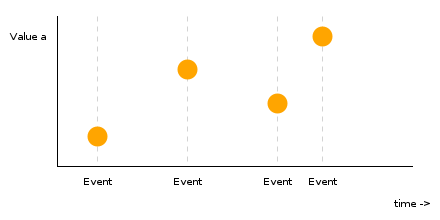
\includegraphics[scale=0.75]{event.png}
  
  {Gambar 2.2.5.1: \emph{Event} pada Reflex}
  \centering
\end{figure}

\emph{Behavior} adalah merupakan penampung dari sebuah nilai, yang dapat berubah seiring berjalannya waktu. \emph{Behavior} selalu memiliki nilai dan apabila suatu nilai dalam \emph{behavior} berubah, maka tidak ada notifikase seperti pada event. Seperti pada contoh dibawah ini, \emph{behavior} dapat berubah nilainya hanya pada saat waktu sebuah \emph{event} terjadi.

\begin{figure}[H]
  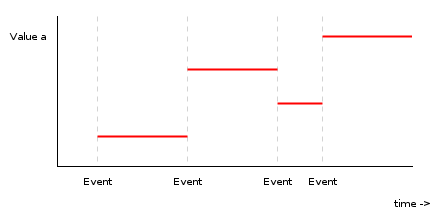
\includegraphics[scale=0.75]{behavior.png}
  
  {Gambar 2.2.5.1: \emph{Behavior} pada Reflex}
  \centering
\end{figure}


Dalam pustaka Reflex, \emph{Dynamic} adalah penampung dari sebuah nilai yang dapat berubah seiring berjalannya waktu dan memungkinkan adanya notifikasi dalam hal terjadinya perubahan. Dengan kata lain, \emph{dynamic} adalah gabungan antara \emph{behavior} dan \emph{event} seperti pada contoh gambar dibawah ini.


\begin{figure}[H]
  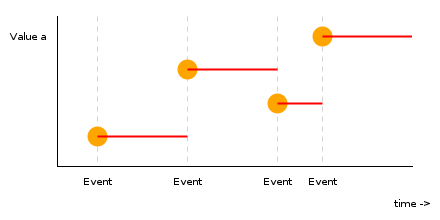
\includegraphics[scale=0.75]{dynamic.png}
  
  {Gambar 2.2.5.1: \emph{Dynamic} pada Reflex}
  \centering
\end{figure}

Konsep \emph{event} dan \emph{dynamic} adalah yang paling sering digunakan dalam pengembangan aplikasi menggunakan pustaka reflex dan pada aplikasi dalam penulisan ilmiah ini.

\section{Pengembangan Aplikasi Desktop GUI dengan Teknologi Web}
Dengan berkembangnya teknologi web di dunia, pengembangan aplikasi desktop GUI yang sebelumnya memerlukan pustaka bawaan masing-masing sistem operasi berubah menjadi pengembangan aplikasi yang menggunakan kombinasi \emph{teknologi web} (dimana komponen utamanya adalah HTML, CSS, Javascript). Penggunaan teknologi web terhadap aplikasi pada desktop menjadi lebih banyak digunakan karena pustaka-pustaka yang ada dapat diintegrasikan secara lintas sistem operasi (dikenal dengan sebutan \emph{cross-platform}).

\subsection{Aplikasi GUI (\emph{Graphical User Interface})}

\emph{Graphical User Interface} atau disingkat GUI adalah antarmuka antara manusia dengan komputer dimana interaksi tersebut menggunakan suatu jendela, ikon dan menu yang dapat dimanipulasikan dengan menggunakan mouse (atau biasanya dapat juga terbatas pada penggunaan \emph{keyboard} saja. [2 http://www.linfo.org/gui.html]

GUI berbeda dengan \emph{command line interfaces} (CLI) yang hanya menggunakan teks dan diakses menggunakan keyboard. Contod dari CLI adalah MS-DOS pada sistem operasi Windows.

GUI pertama kali ditemukan oleh Vannevar Bush, seorang ilmuwan yang bekerja di Massachussetts Institute of Technology (MIT) saat Perang Dunia II. Pada tahun 1963, lulusan MIT bernama Ivan Sutherland mengembangkan sebuah program bernama Skecthpad yang memungkinkan pengguna untuk melakukan manipulasi langsung terhadap suatu objek gambar pada sebuah layar CRT menggunakan pena sederhana.

Pengembangan GUI meningkat dengan pesat ditahun 1970, dimana perusahaan Xerox membuat sebuah komputer bernama PARC yang dirilis tahun 1974. PARC menjadi inspirasi banyak pengembang pemrograman GUI salah satunya adalah Steve Jobs.

\subsection{Teknologi Web Dengan Bahasa Haskell}
Sebagaimana telah di sebutkan pada sub bab sebelumnya, Haskell memungkinkan pengembang mengetahui lebih dahulu apabila adanya error terhadap kode program. Konsep pemrograman fungsional pada Haskell tersebut sangat baik apabila diterapkan untuk membuat aplikasi dengan menggunakan teknologi web, dimana pemrograman dengan teknologi web tidak memungkinkan pengembang untuk mengetahui error kode sebelum aplikasi dijalankan.

Dalam pengembangan aplikasi berbasis teknologi web menggunakan Haskell, pustaka yang digunakan adalah pustaka Jsaddle dan Reflex-Dom. Jsaddle merupakan pustaka yang menjadikan seluruh komponen pada kode program dapat dikompilasi menjadi kode beberapa komponen kode pada teknologi web dengan menggunakan GHC. Reflex-Dom adalah pustaka yang menghubungkan \emph{Document Object Model} (DOM) kedalam lingkup FRP yang ada pada Reflex untuk kemudian hasilnya akan diterjemahkan kedalam salah saut komponen teknologi web yaitu bahasa Javascript.

\subsubsection{\emph{Hypertext Markup Language} atau HTML}
HTML merupakan sebuah blok dasar pembangun teknologi Web yang berfungsi untuk menggambarkan atau menampilkan konten dari sebuah website. \emph{Hypertext} pada HTML mengacu pada tautan yang menghubungkan satu halaman web dengan halaman web lainnya, baik dalam situs tunggal maupun antara beberapa situs. Tautan merupakan aspek fundamental dari sebuah Web. Dengan mengunggah konten kedalam internet dan menautkannya dengan halaman yang dibuat oleh orang lain, maka peengembang situs telah secara aktif menjadi partisipan dalam \emph{World Wide Web}.

HTML menggunakan \emph{Markup} untuk mengindikasikan teks, gambar, dan konten lain yang akan ditampilkan di sebuah Web \emph{browser}. \emph{Markup} dalam HTML termasuk didalamnya adalah $<$head$>$, $<$title$>$, $<$body$>$, $<$header$>$, dan lain-lain. Dengan demikian, HTML bukanlah merupakan bahasa pemrograman melainkan sebuah bahasa \emph{markup} yang digunakan untuk memberitahukan sebuah browser mengenai cara menampilkan sebuah situs yang dikunjungi oleh pengguna Web browser.

HTML memiliki 4 (empat) elemen dasar, yaitu: a) tag pembuka (\emph{opening tag}), b) tag penutup (\emph{closing tag}), c) konten dan d) element (gabungan dari a, b dan c). Dilihat dari kategorinya, elemen pada HTML terbagi kedalam 2 (dua) kategori yaitu:
\begin{enumerate}
\item \emph{Block level element}
  \emph{Block level element} membentuk sebuah blok pada halaman situs dan tampak pada baris baru setiap elemennya. \emph{Block level element} cenderung berupa elemen terstruktur pada sebuah halaman situs yang merepresentasikan sebuah paragraf, catatan kaki, menu navigasi.
\item \emph{Inline element}
  \emph{Inline element} adalah elemen yang berada diantara \emph{Block level element} dan melingkupi sebagian kecil dari konten yang berada diantara \emph{Block level element}. \emph{Inline element} biasanya tampil diantara paragraf yang berada di dalam sebuah \emph{Block level element}.
\end{enumerate}

Elemen juga dapat memiliki atribut yang berisikan tambahan informasi mengenai elemen yang memiliki kekhususan dibandingkan elemen normal lainnya. Sebuah atribut pada HTML harus memuat paling sedikit:
\begin{enumerate}
\item Spasi antara atribut dengan nama elemen (atau dengan atribut yang sudah ada sebelumnya)
\item Nama atribut, diikuti dengan tanda sama dengan (=)
\item Tanda petik diantara nilai dari atribut yang diinginkan
\end{enumerate}
Hal diatas dikecualikan pada atribut bertipe boolean, dimana dalam penulisannya tidak memerlukan tanda sama dengan (=).

Secara umum, anatomi dari sebuah dokumen HTML adalah sebagai berikut:\\
  \begin{lstlisting}[language=HTML]
    <!DOCTYPE html>
    <html>
      <head>
        <meta charset="utf-8">
        <title>Judul Website</title>
      </head>
      <body>
        <p>Ini adalah contoh</p>
      </body>
    </html>
  \end{lstlisting}
Dari struktur diatas, elemen-elemen dasar dari sebuah dokumen HTML antara lain:
\begin{enumerate}
\item $<$!DOCTYPE html$>$ : Penanda bahwa dokumen tersebut merupakan dokumen HTML
\item $<$html$>$$<$/html$>$ : Merupakan elemen utama dari halaman web yang membungkus elemen-elemen HTML lainnya
\item $<$head$>$ $<$/head$>$ : Merupakan bagian pada HTML yang konten diantara tanda pembua dan penutupnya tidak akan ditampilkan pada layar pengguna.
\item $<$meta charset="utf-8"$>$ : Elemen ini mengharuskan karakter yang tampil menggunakan standarisasi utf-8
\item $<$title$>$ $<$/title$>$ : Elemen yang akan menampilkan judul pada website di browser
  \item $<$body$>$ $<$/body$>$ : Isi utama dari halaman web. Elemen ini mengandung seluruh konten yang ingin ditampilkan pengembang aplikasi kepada pengguna.
\end{enumerate}

\subsubsection{\emph{Cascading Style Sheet} atau CSS}
CSS digunakan untuk memberikan gaya dan layout pada satu atau lebih halaman web dengan cara memanipulasi atribut-atribut pada elemen HTML. Cara kerja CSS adalah dengan diaplikasikannya ketentuan-ketentuan yang ditulis oleh pengembang pada file CSS oleh browser. Ketentuan CSS antara lain:
\begin{enumerate}
\item Kumpulan properti yang akan digunakan untuk memperbaharui cara konten HTML disajikan.
\item Kumpulan penyeleksi yang akan digunakan untuk menandai sebuah element dimana pembaharuan atas sebuah properti tersebut diinginkan.
\end{enumerate}
Secara garis besar, browser akan mentranslasikan HTML dan CSS kedalam DOM untuk kemudian dilakukan penggabungan antara HTML dan CSS dan akhirnya DOM hasil penggabungan tersebut ditampilkan oleh browser kedalam layar browser tersebut.

\subsubsection{Javascript}

Javascript adalah sebuah bahasa \emph{scripting} berorientasi objek. Javascript dapat dihubungkan kedalam sebuah objek yang ada dilingkungannya untuk memberikan sebuah kontrol program terhadap objek tersebut.

Pada penulisan ini, akan digunakan \emph{client-side} Javascript, yaitu Javascript yang memberikan kemampuan terhadap objeknya untuk melakukan kontrol terhadap sebuah browser dan DOM. Javascript pada sisi klien memudahkan pengembang untuk menempatkan elemen-elemen pada HTML dan merespon kejadian (\emph{event}) yang dibuat oleh pengguna seperti menekan mouse, form input, dan lain-lain.

\subsubsection{Penggunaan Reflex-Dom Sebagai Metode FRP untuk Teknologi Web}

Reflex-Dom sebagaimana telah dijelaskan sebelumnya adalah pustaka yang menggunakan pustaka Reflex untuk memanipulasikan sebuah DOM pada HTML dengan menggunakan metode FRP. Fungsi-fungsi yang terdapat pada Reflex-Dom memungkinkan pengembang untuk mendefinisikan komponen teknologi web yaitu HTML dan Javascript. Pendefinisian yang dilakukan tersebut adalah dengan cara menyesuaikan output dari setiap fungsi pada Reflex-Dom dengan komponen-komponen HTML sehingga manipulasi fungsi yang ditulis dengan bahasa pemrograman Haskell dapat ditranslasikan oleh GHC kedalam file berisikan kode bahasa pemrograman Javascript ketika dikompilasi oleh GHC.

Sebagai contoh, berikut ini adalah potongan kode program pada haskell yang kemudian akan diterjemahkan kedalam bahasa Javascript untuk membuat DOM yang akan ditampilkan kedalam HTML:\\

  \begin{lstlisting}[language=Haskell]
    {-# LANGUAGE OverloadedStrings #-}
    import Reflex.Dom

    main :: IO ()
    main = mainWidget $ el "h1" $ text "Selamat datang di Reflex-Dom"
  \end{lstlisting}
  akan diterjemahkan kedalam DOM pada HTML menjadi sebagai berikut:
\\
  \begin{lstlisting}[language=HTML]
    <html>
      <head>
      </head>
      <body>
        <h1>Selamat datang di Reflex-Dom</h1>
      </body>
    </html>
  \end{lstlisting}
  kode HTML diatas diterjemahkan melalui Javascript sebagai perantara transalasi sebuah DOM.

  Dari potongan kode diatas, maka pengembang mengetahui bahwa sebuah fungsi main pada Haskell dimana terdapat tipe \fhaskell{IO ()} adalah fungsi yang memungkinkan adanya interaksi dengan dunia luar. Fungsi main tersebut juga merupakan hasil dari kombinasi beberapa fungsi diantaranya \fhaskell{mainWidget, el, text}. Masing-masing fungsi tersebut memiliki Tipe Fungsi sebagai berikut:\\
    \begin{lstlisting}[language=Haskell]
       el   :: Text -> m a -> m a
       text :: Text -> m ()
       mainWidget :: Widget Spider (Gui Spider (WithWebView SpiderHost) (HostFrame Spider)) () -> IO ()
    \end{lstlisting}

    Dari tipe fungsi diatas, penjelasannya adalah sebagai berikut:
    \begin{enumerate}
    \item \emph{m} adalah merupakan sebuah tipe data monadik yang serupa dengan IO. Hanya saja pada notasi ini, \fhaskell{m} digambarkan sebagai suatu abstraksi dalam pemrograman Haskell.
    \item Text merupakan tipe data Text.
    \item Spider merupakan satuan waktu pada pustaka Reflex dimana dalam konsep FRP, waktu digunakan untuk menentukan event dan behavior.
    \item SpiderHost merupakan tempat dimana waktu dicatat.
    \item HostFrame merupakan kerangka dari sebuah Host untuk menampung sebuah waktu.
\end{enumerate}
    Pada pembuatan Aplikasi, fungsi-fungsi pada reflex-dom akan digunakan sebagai fondasi utama yang akan mentranslasikan lingkungan fungsional reaktif kedalam DOM yang merupakan bagian dari HTML. Diantara fungsi-fungsi yang terdapat di dalam referensi cepat (\emph{quick reference}) yang tertulis dalam dokumentasi resmi pustaka reflex [3 https://github.com/reflex-frp/reflex-dom/blob/develop/Quickref.md], penggunaan fungsi-fungsi yang secara umum digunakan dalam pembuatan sebuah aplikasi adalah sebagai berikut:\\

    \begin{enumerate}
    \item el dan el'
    \item elAttr dan elAttr'
    \item elDynAttr dan elDynAttr'
    \item elClass
    \item text
    \item dynText
    \item display
    \item button
    \item blank

    \end{enumerate}

    Dalam pustaka reflex-dom, terdapat gaya penulisan fungsi untuk memudahkan pengembang dalam mengetahui kegunaannya yaitu dengan pembubuhan tanda \fhaskell{'} pada akhir sebuah fungsi dan penambahan kata \fhaskell{Dyn} atau \fhaskell{dyn} pada fungsi tersebut. Contoh mendasar dari penggunaan tanda \fhaskell{'} adalah pada fungsi \fhaskell{el} dan \fhaskell{el'}, kemudian \fhaskell{text} dan \fhaskell{dynText} untuk penambahan kata \fhaskell{dyn} pada sebuah fungsi.

    Untuk mengetahui perbedaan mendasar dari \fhaskell{el} dan \fhaskell{el'} (atau fungsi lain pada reflex-dom yang serupa), dapat dilihat dari tipe fungsinya masing-masing. Fungsi \fhaskell{el} memiliki tipe fungsi \fhaskell{el :: Text -> m t a -> m t a} dan fungsi \fhaskell{el'} memiliki tipe fungsi \fhaskell{el' :: Text -> m t a -> m t (El, a)}. Dari tipe fungsi tersebut, diketahui bahwa fungsi \fhaskell{el'} akan mengembalikan sebuah nilai \fhaskell{m t (El,a)} dimana \fhaskell{El} adalah sebuah elemen pada DOM. Sehingga penggunaan fungsi \fhaskell{el'} adalah pada kondisi dimana kita ingin mengambil nilai \fhaskell{El} pada sebuah DOM untuk dilakukan manipulasi kemudian.

    Penambahan kata \fhaskell{Dyn} atau \fhaskell{dyn} pada sebuah fungsi bertujuan untuk membedakan antara fungsi yang akan menghasilkan elemen statis dan elemen dinamis. Statis dan dinamis tersebut berada dalam konteks FRP, dimana dinamis dapat diartikan bahwa elemen tersebut nilainya akan berubah seiring dengan waktu sedangkan statis tidak akan berubah selamanya. Hal ini dapat dilihat dalam tipe fungsi \fhaskell{text :: Text -> m t ()} dan \fhaskell{dynText :: Dynamic t Text -> m t ()} dimana fungsi \fhaskell{dynText} memiliki tipe parameter yang terbungkus dalam tipe data \fhaskell{Dynamic}. Tipe data \fhaskell{Dynamic} menandakan bahwa parameter tersebut berada dalam konteks FRP. Perbedaan tipe fungsi sangat memudahkan pengembang untuk merancang sebuah aplikasi yang mana didalamnya ada elemen-elemen yang sifatnya \emph{immutable} dan \emph{mutable}.

    Fungsi lain yang banyak digunakan adalah fungsi \fhaskell{button :: Text -> m (Event ())} dimana parameter pertama dari fungsi tersebut adalah nama dari \emph{button} yang dibuat dan hasil keluaran dari fungsi tersebut adalah sebuah \emph{event} yang berada pada sebuah tipe data monadik. Dari hasil keluaran tersebut, fungsi \fhaskell{button} akan melakukan sebuah \emph{trigger} untuk memanipulasi element pada DOM atau fungsi lain yang membutuhkan parameter \fhaskell{Event}.


\subsection{Pustaka JSaddle Sebagai Pendukung Pengembangan Aplikasi Desktop GUI dengan Teknologi Web}
Pustaka JSaddle merupakan sebuah pustaka antarmuka untuk bahasa pemrograman Javascript yang bekerja pada GHCJS (kompiler Haskell ke Javascript) maupun GHC. Pada saat kode Haskell dikompilasi dengan GHC, JSaddle menggunakan pustaka ghcjs-dom sebagai acuannya. Pada penulisan ini, bagian dari pustaka JSaddle yang digunakan adalah pustaka jsaddle-wkwebview, dimana JSaddle akan dihubungkan dengan pustaka WkWebView yang disediakan oleh sistem operasi MacOS.



\end{document}

